\chapter{Experimental Setup}
\label{chapter: experimental setup}

% Small introduction to the chapter,
% Briefly touch on reproducibility, comparisons with existing methods, etc.

% \ednote{Change "usage data" to "Interpretation data" OR "Estimation data"}
% \ednote{Get a set of "terminologies" for all important parts.}
% \ednote{Explain some things LESS concisely, giving a more "step by step" explanation.}

This chapter outlines the testing setup and introduces specific terminology for the collected data.
A precise vocabulary and understanding of the data characteristics are essential to create effective test and training sets for the comparative SoA Deep Learning interpretation system.
Therefore, this chapter discusses the testing setup (see \cref{section: experimental setup - testing setup}), the specific vocabulary for, and characteristics of, the collected data set (see \cref{section: experimental setup - dataset}).
Lastly, this chapter presents the training and test sets we used for the comparative model, as well as a reasoning for these choices (see \cref{section: evaluation - baseline analysis}).

% \ednote{Why are we doing this?\\ What are we testing and why, refer back to my research question number 3\\ This is the setup used for the evaluation}
% 
% \ednote{ The previous might make this paragraph un needed}
% 
% This chapter presents the physical setup, the hardware used, and the testing procedures in \cref{section: experimental setup - testing setup}.
% The collected data is discussed in \cref{section: experimental setup - dataset}, and some general terminology to refer to this data is established.
% Lastly, we present and substantiate the choice of comparison model in \cref{section: experimental setup - baseline analysis}.
% \Cref{chapter: evaluation} provides a further analysis of this comparison.



\section{Testing Setup}
\label{section: experimental setup - testing setup}

%     -[[ Hardware Setup ]]-
% - What exact chip do we use, what exact Kinect
% - What firmware do we run, and why
% - refer to the appendix with more in-depth info
% - 
% FMCW
The mmWave~radar used in this thesis is the IWR6843ISK by Texas~Instruments.
The radar requires firmware to run, a diverse variety of which are provided by Texas Instruments, for varying sensing tasks.
% The radar runs firmware, a variety of which are provided by TI, for various sensing tasks.
% This chip needs to run a specific firmware to work; TI provides a set of ready-made firmware, which differ slightly in what they provide to the end user.
The main firmware characteristics that are important to this thesis are the number of points generated, the signal-to-noise ratio, and the discriminative value of each point, for arm angle estimation.
% For this thesis, a "useful" point can tell you a lot about the position of a (semi-static) arm.
We chose the \textit{Mobile Tracker} firmware~\cite{ti_mmwave_firmware} as it meets those criteria.
% These criteria were met by the \textit{Mobile Tracker} firmware~\cite{ti_mmwave_firmware}. 
% For this reason, and the fact that the firmware aligned well with an interpretation method which was being explored at the time, this became the firmware of choice.
For a more detailed discussion of this firmware choice, see Appendix~\ref{appendix: configuration in detail}.
% Kinect
In addition to the mmWave Radar, a Kinect 2 was used to collect ground truth data.
The skeletal estimation was generated through a code base published by Kharche on GitHub~\cite{kharche2019skeletal}, which creates a smooth skeletal estimation and saves it, along with timestamps, to a CSV file.
This skeletal estimation was transformed into an arm angle estimation by calculating the angle of the vector going from the \textit{neck keypoint} to either \textit{wrist keypoint}, with regards to the down vector, see \cref{figure: kinect angle}.

\begin{figure}[!htb]
    \centering
    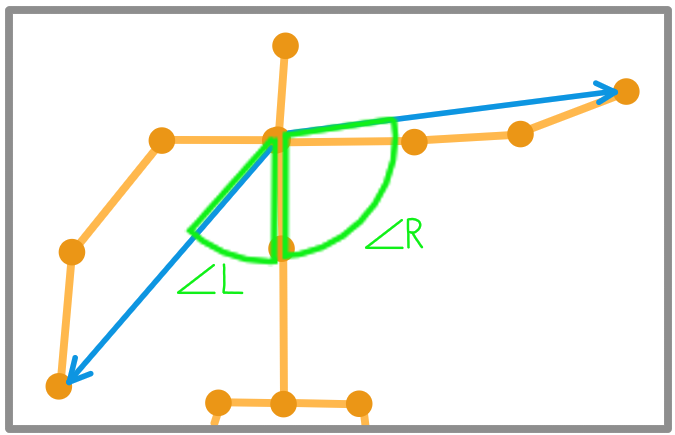
\includegraphics[width=0.5\linewidth]{figures/internal data/gt angle calculation diagram.png}
    \caption{Skeletal estimation into Arm Angle estimation visualisation.}
    \label{figure: kinect angle}
\end{figure}

\begin{figure}[!htb]
    \centering
    \begin{subfigure}{0.45\textwidth}
       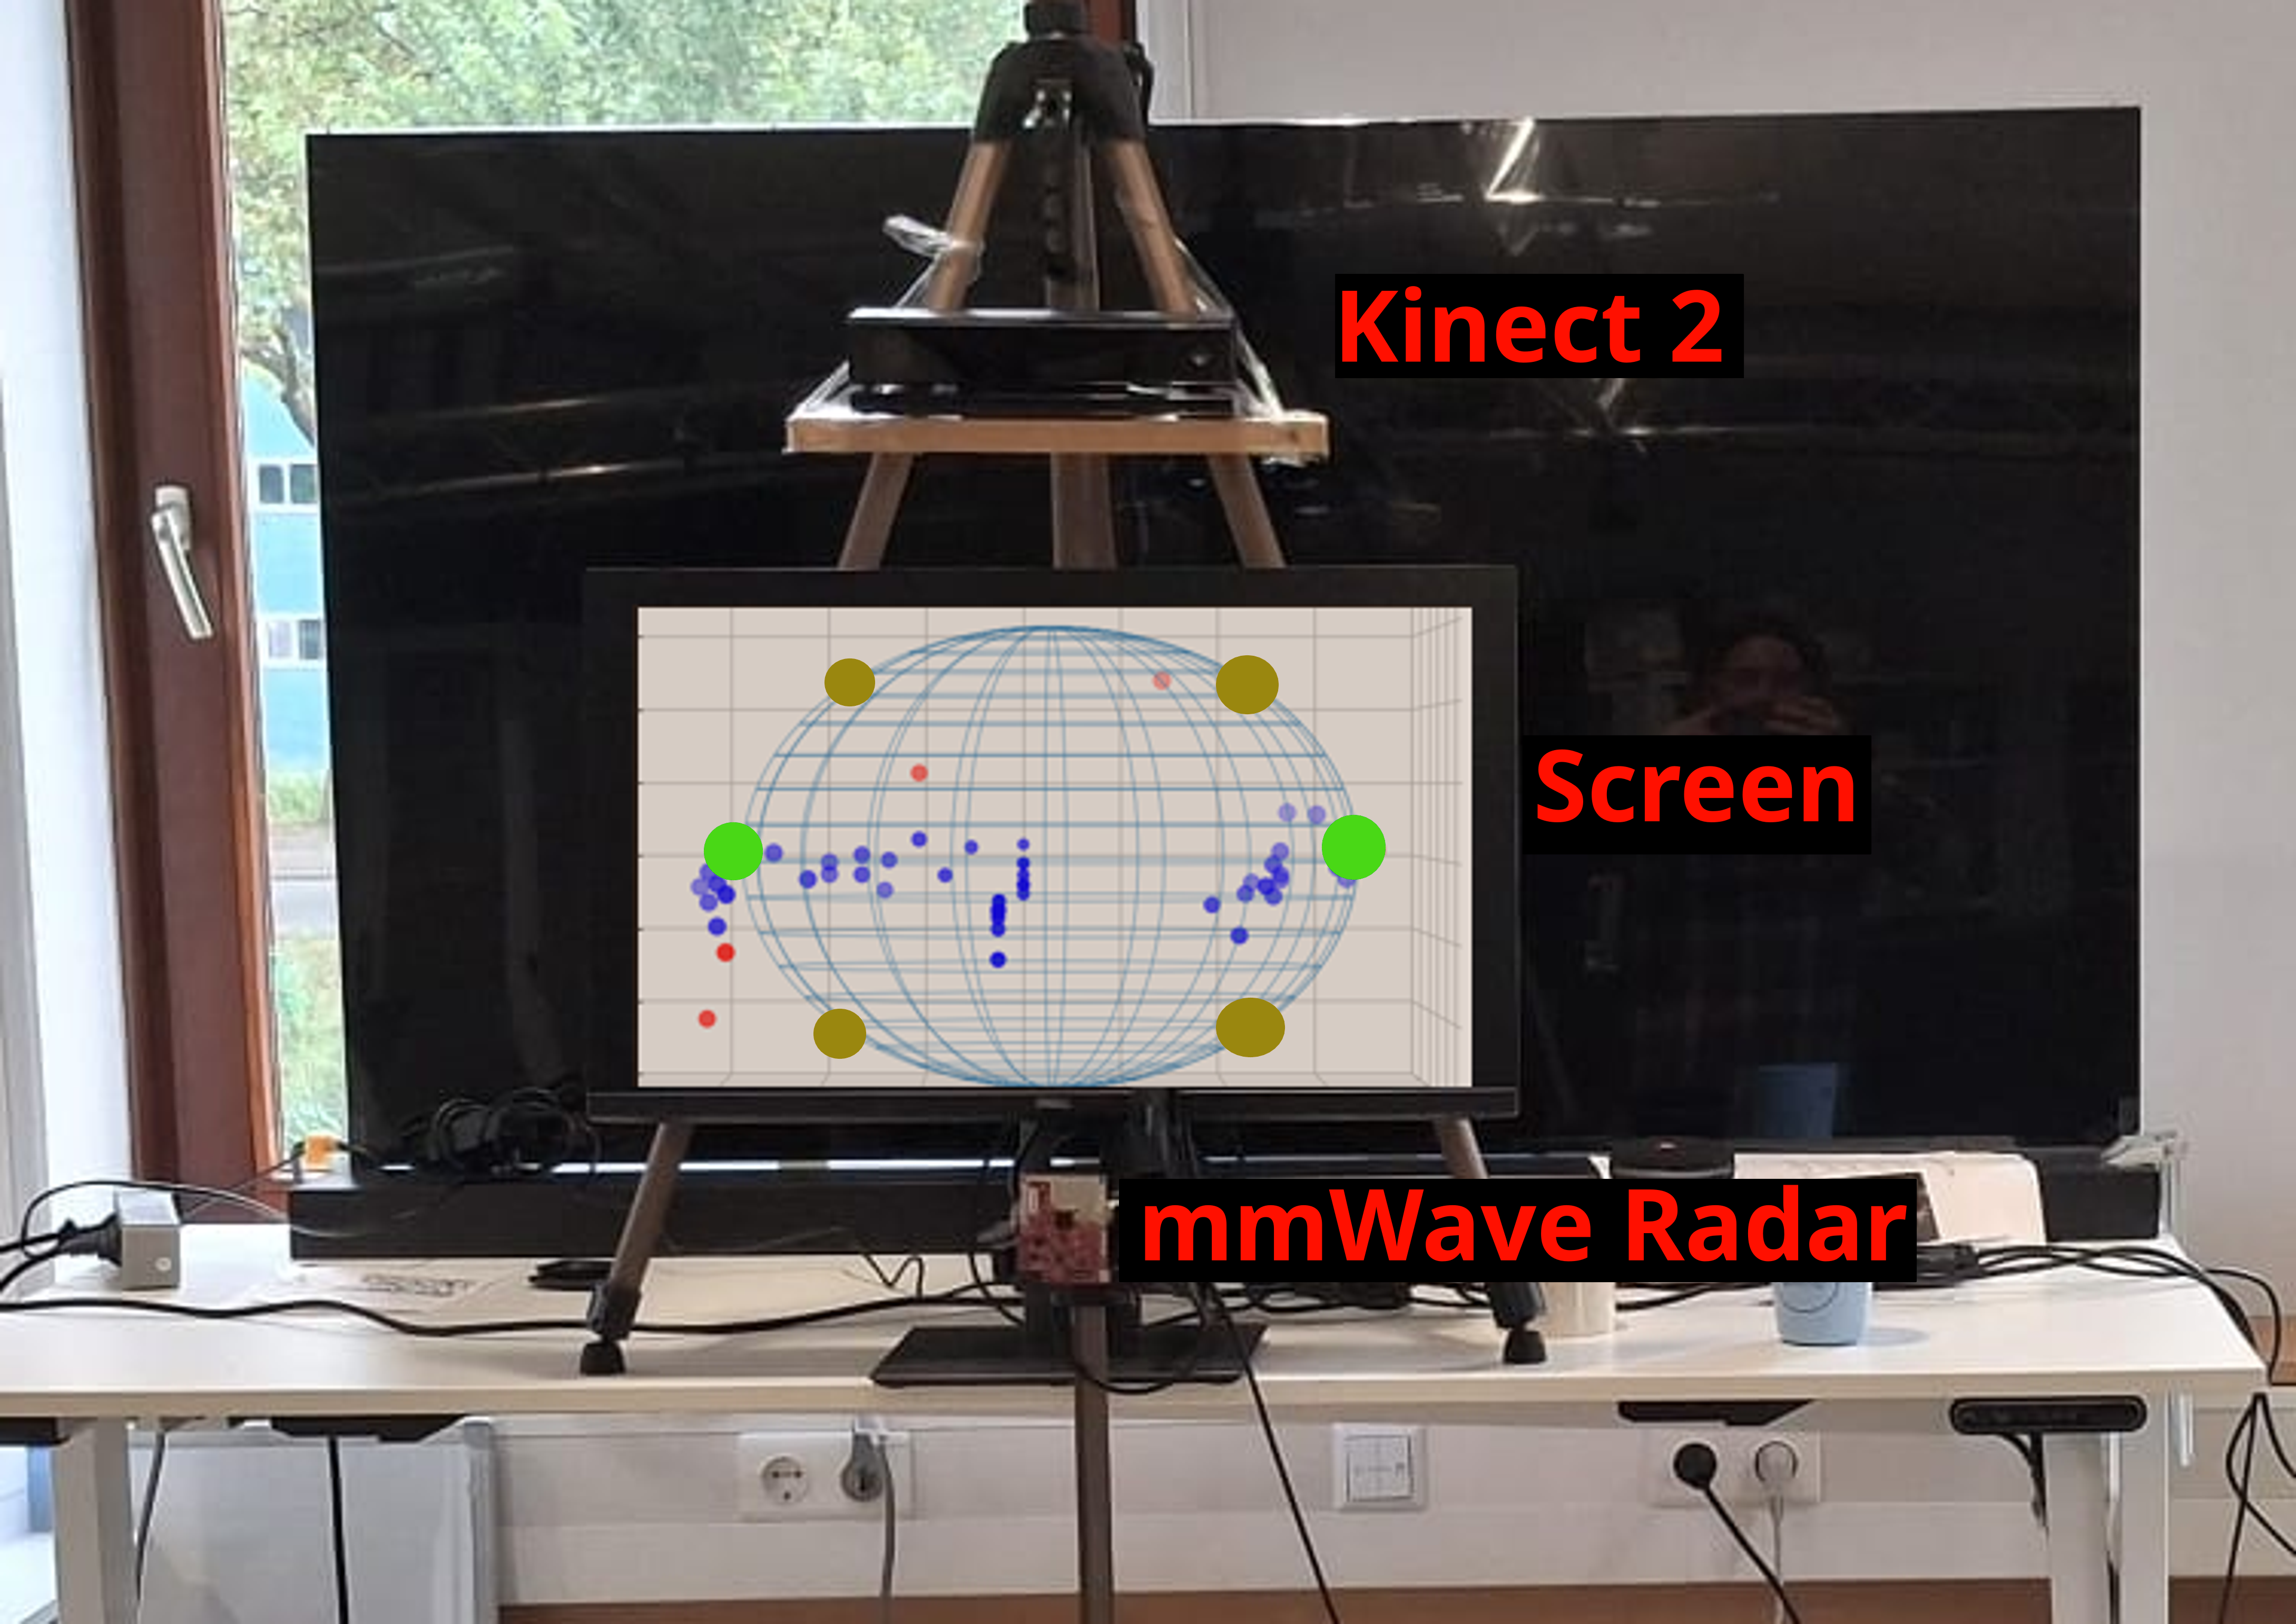
\includegraphics[width=1\textwidth]{figures/experimental setup/sensor view edit.png}
       \caption{User view}
    \label{figure: testing environment - user view}
    \end{subfigure}
    \hfill
    \begin{subfigure}{0.45\textwidth}
       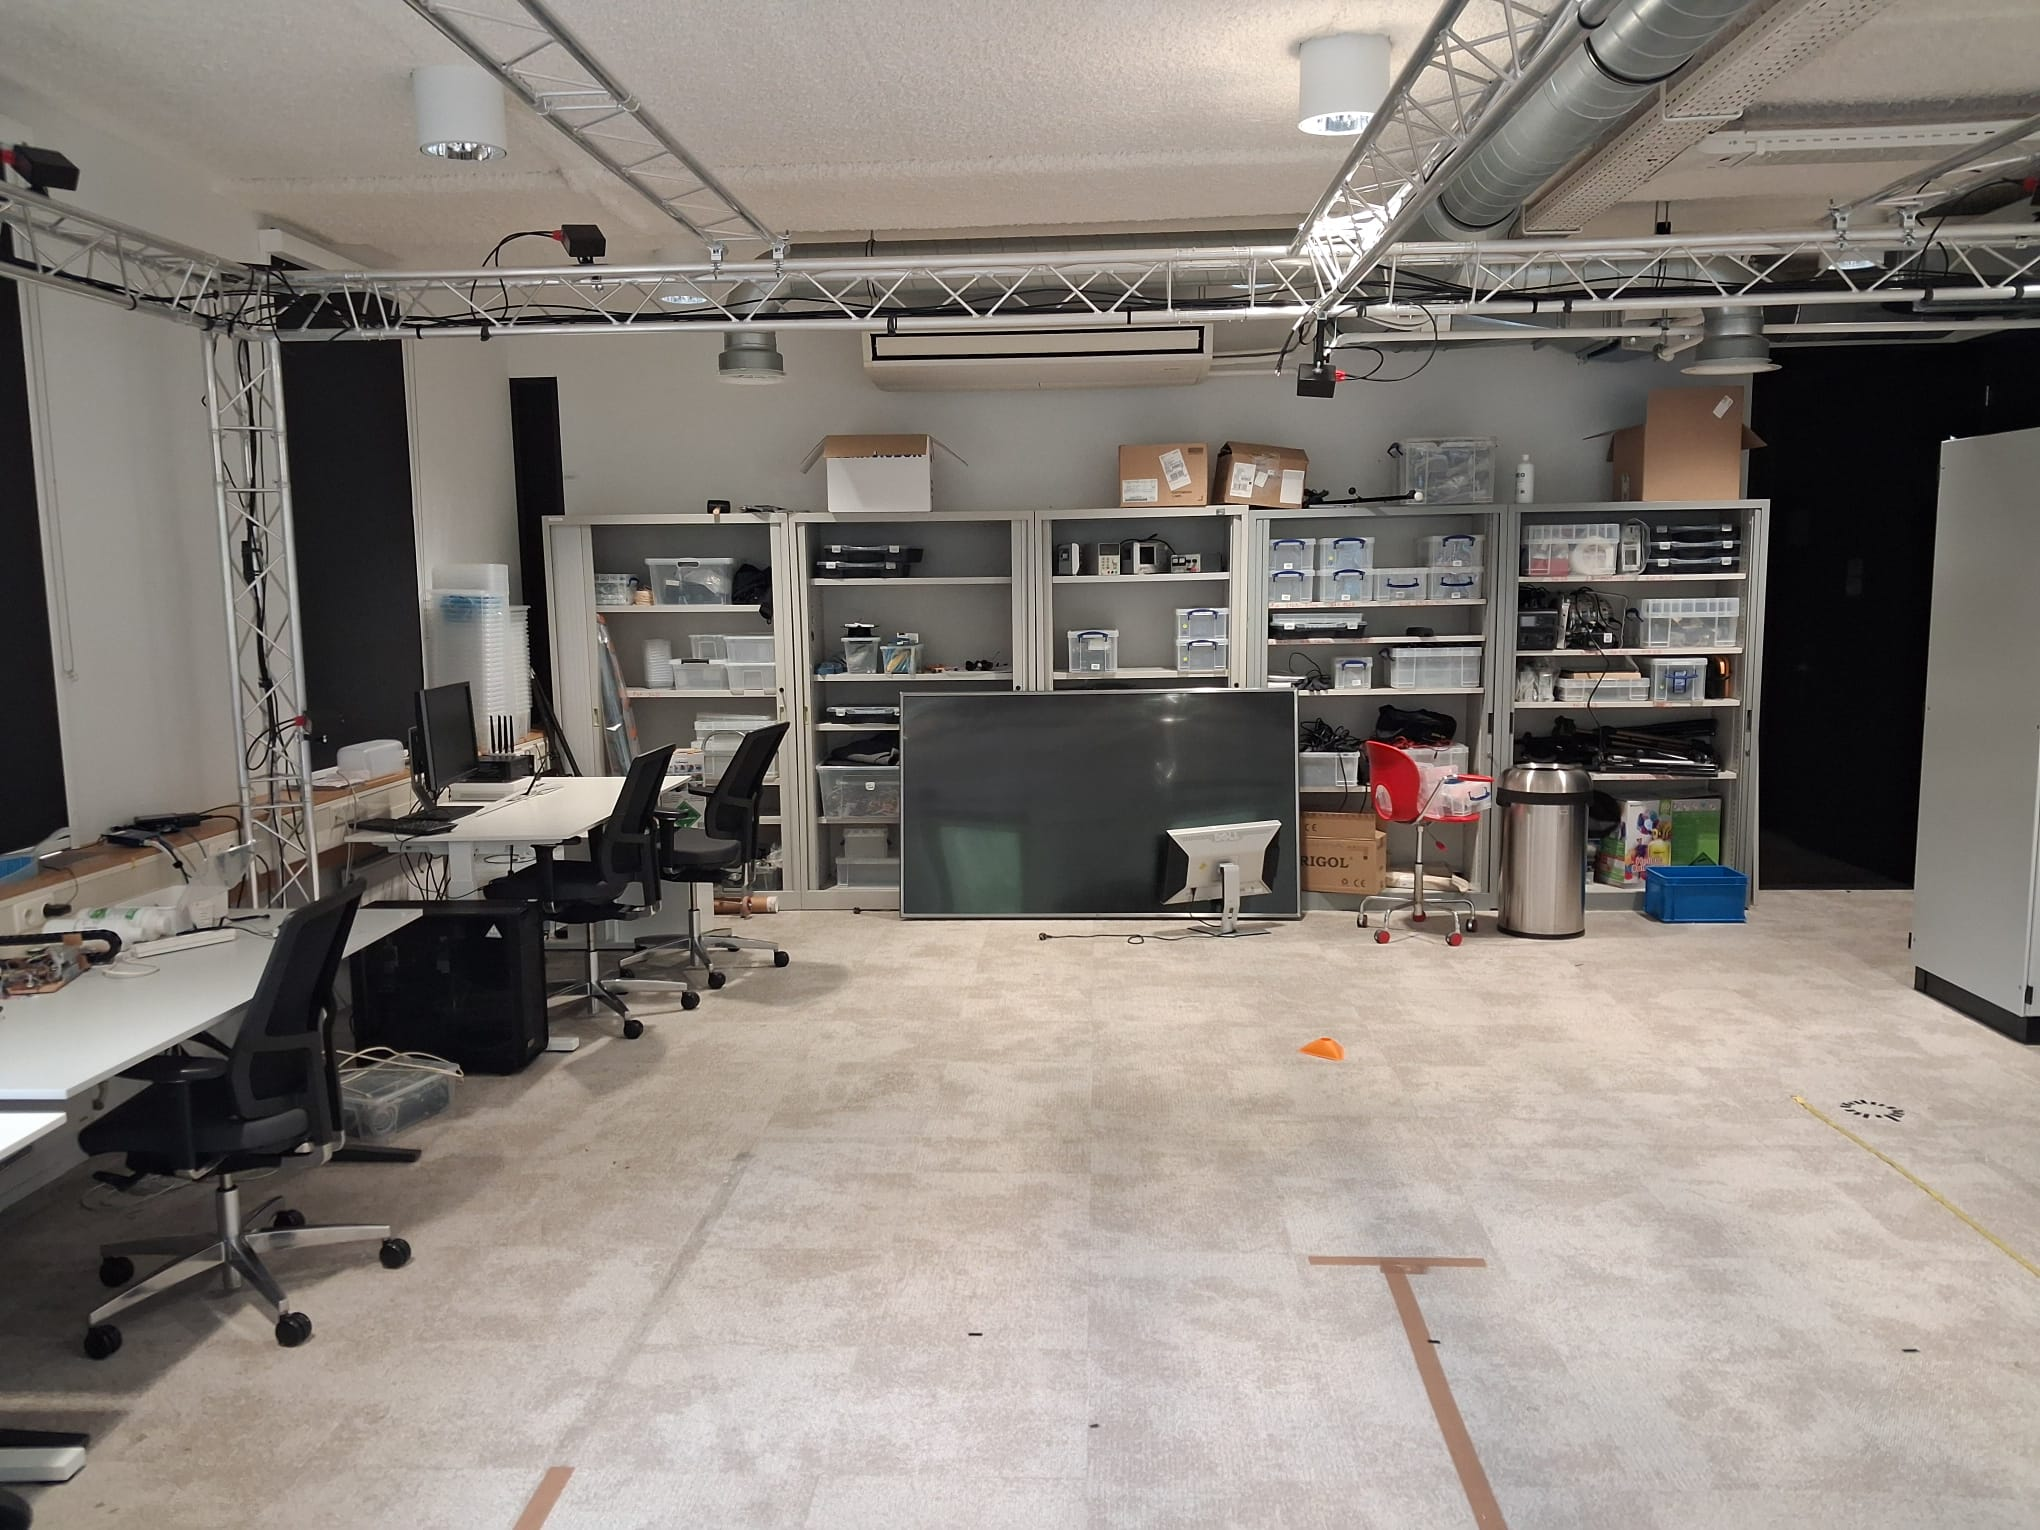
\includegraphics[width=1\textwidth]{figures/experimental setup/room_view.jpeg}
       \caption{View from the Sensor's perspective}
       \label{figure: testing environment - sensor view}
    \end{subfigure}
    \caption{The testing environment, providing the user view (a) and the sensor's perspective (b).}
    \label{figure: testing environment}
\end{figure}

%     -[[ Physical setup ]]-
% - What does the room look like
%   - Where was the sensor
%   - Where was the user
% - What effect could the room setup have
% - 
The experiments are performed in a large open room ($7 \times 10$~m). 
The mmWave~radar was mounted at a height of 125~cm and was tilted upwards at an angle of $5\degree$.
The Kinect was mounted at a height of 175~cm with an angle of $5\degree$ downwards.
The user could see a real-time visualisation of the incoming point cloud, as well as the current arm angle estimation on a screen in front of them, as shown in \cref{figure: testing environment - user view}.
% A screen was also present, on which the user could see their currently predicted zones, and the incoming point clouds.
The user was standing at a distance of 2 meters from the sensors.
Appendix \ref{appendix: experimental setup} shows the experimental setup in detail.
A large and open room was used, see \cref{figure: testing environment - sensor view}, which meant that back wall reflections were spatially distinct from the user.
This resulted in point clouds with relatively little noise, producing a relatively high-quality dataset.
% \ednote{Info about the back wall is not needed and only confusing}
% The back wall was also broken up with open shelving, diffusing any potential backscatter.
% % which should've scattered the incoming millimeter waves, as opposed to reflecting them.
% The large screen at the end of the room was angled upwards, reflecting the mmWaves away from, rather than back at, the radar.
% % The large screen present was angled upwards, and would've thus not reflected the signal to the mmWave sensor.
% These factors resulted in the mmWave radar producing point clouds with relatively little noise in this room, which in turn reduced the need for aggressive noise reduction, creating a higher-quality dataset.
% % meant that the noise reduction algorithms did not have to be tuned as much.



%     -[[ Testing procedures]]-
% - How was the user informed
% - What were they asked to do
% - How did we provide feedback
% - Refer to the appendix for more in-depth info
% - 

Six users took part in this experiment.
For each user, we collected between 4 and 7 recordings; the average duration of a recording is 140 seconds.
Each recording consists of two distinct parts: the \textit{calibration} part, and the \textit{interpretation} part.
The \textit{calibration} had an average duration of 20 seconds, during which the user moved their arms up and down. % along their body.
The remainder of the recording is part of the \textit{interpretation}, and has an average duration of 120 seconds.
During the \textit{interpretation}, the user moves their arms to a specific position and holds the position for a few seconds before moving their arms to the next position.
% The whole experiment consisted of between 4 and 7 recordings per user.
% During these recordings, the users
% , took between 20 and 40 minutes.
During the recordings, both the mmWave radar point cloud and a skeletal estimation produced by the Kinect 2 were recorded.
The Kinect 2 recorded a video channel, but this video channel was only used to create the skeletal estimate and was never saved.
While in use, the system produced musical notes in accordance with the pose that the system predicted at that given time.
The users were given a consent form before the experiment, and were allowed to drop out of the experiment at any point.
For privacy reasons, we chose only to record the height and arm span of the users, and no other information, see Appendix~\ref{appendix: user information}.
Before the experiment took place, we informed the users of how the system worked and what was expected of them through an explanatory PDF (see Appendix~\ref{appendix: user explanation}).
The specific actions the users performed are discussed in \cref{section: experimental setup - dataset}.

% \ednote{Briefly explain the general testing situation, "how many people did we have", "how long roughly did each test take", and also "what data do we record", and the fact that the users hear the music output.\\ Briefly mention (and forward references to explanation) how many standard recordings and free play people had, and roughly how long they took.}
% \ednote{Specify that we did not make any user interviews, briefly mention our privacy concern stuff.}
 % Users were informed of how the system worked and what they were expected to do through an explanatory PDF (see Appendix~\ref{appendix: user explanation}).
% The specific actions the users performed will be discussed in \cref{section: experimental setup - dataset}.
% \ednote{This "advice part" can mostly be skipped/removed.}
% After each recording, the researcher provided some guidance to the user about how to best use the system, based on the user error observed in the previous recording.
% Common advice included keeping consistent micro-movements in the hands to increase the point cloud stability and density in those regions.
% Furthermore, a more precise specification of the exact \textit{spatial regions} which correlated to a specific \textit{arm position} ("low", "middle", or "high") was also often given as advice.
% % Commonly given advice was to wave their hands, or do "jazz hands", as well as informing the user where the optimal "zone positions" are (for low, mid, high).
% A more detailed overview of the provided feedback, along with notes of the user performance, can be found in Appendix \ref{appendix: experiment notes}.


%     -[[ ]]-
% - 
% - 
% - 
%     -[[ ]]-

% Double separation line and spacing
% \vspace{2em}
% \hrule
% \vspace{0.2em}
% \hrule
% \vspace{2em}

%     [[ Hardware setup (chip, firmware, config ]]
% Describe the chip we used, the config we used on that chip, the reason for that choice, the specific config used.
% Also, describe the method for ground truth collection.

% The mmWave radar used for this thesis was the IWR6843ISK by Texas Instruments.
% The firmware which is used on this chip is the \textit{Mobile Tracker} firmware \cite{ti_mmwave_firmware}, in part chosen due to it producing a reasonable number of relatively representative points, and in part due to legacy reasons, which are further discussed in Appendix \ref{appendix: configuration in detail}.
% Next to this, a Microsoft Kinect 2 was used to collect the ground truth.
% To get a skeletal estimation from the Kinect, a code base by \citeauthor{kharche2019skeletal}\cite{kharche2019skeletal} was used.
% This code base could record the skeletal estimation produced by the Kinect to a CSV file, with timestamps for each frame, making it a good choice for the ground truth.


%     [[ Hardware setup p2. ]]
% Discuss the specific firmware used, what the advantages and disadvantages are, and what other options we might have had.
% -- [ SKIP ] -- 

%     [[ Environment setup (mounting, space) ]]
% Describe the room in which the tests were held, describe the positions for the various sensors, as well as the position of the user
% Use photos, specify measurements/distances

% [[ Testing procedure ]]
% Describe the testing procedure.
% Describe the types of data that were collected and why,
% Describe the way in which the user was guided.

% Explain the type of room we took measurements in and why, also describe the sensors we use (fmcw + kinect)

% Describe the test setup specifically, use photos and specify measurements (user stood at a distance of 2m)

% Explain the testing procedure, what did we tell the users?


\section{Dataset}
\label{section: experimental setup - dataset}




\subsection*{Frame specification}
\begin{figure}[!htb]
    \centering
    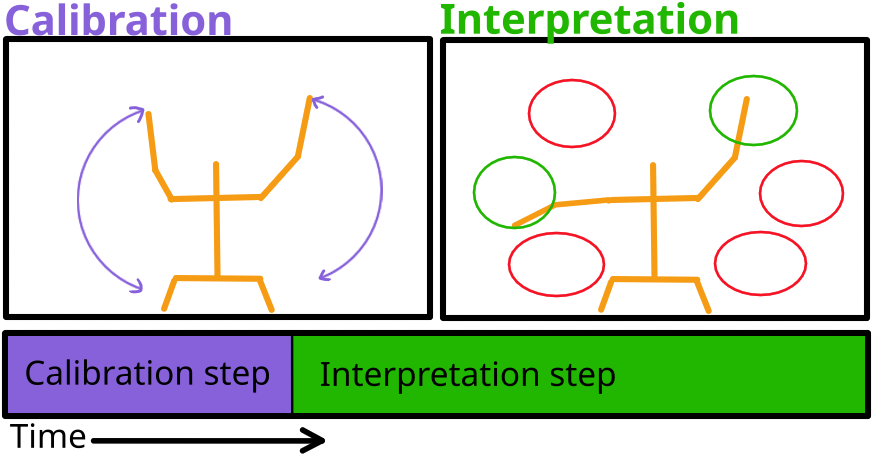
\includegraphics[width=0.7\linewidth]{figures/experimental setup/calibration vs estimation diagram.png}
    \caption{Visualisation of the two frametypes present in each recording}
    \label{fig:frame_types}
\end{figure}


% \ednote{Have an explaining asterix (*) telling why we don't use "Train/Test" as our data terms, cause this gets confusing later on with mars (As we train mars on the "IAmMuse test" data).}
% \ednote{Explain more clearly that EVERY recording has BOTH calib and usage data,}



%       -------------------------------
%     [[ Frame-by-frame data structure ]]
%       -------------------------------
% - Explain the division between "initialization frames" and "usage frames", why this is important, and how this specification is made (timestamp at MEB initialization).
% - Explain the different characteristics of these two types of frame data (initialization has both hands at the same time)
% - Mention that this "initialization" is on a \textit{recording-by-recordings} basis
% - Refer to the frame count appendix

To properly compare IAmMuse to the state-of-the-art solutions, a clear definition of the available data is required.
% We'll need a clear specification of the data that is available.
% Frame specification
First, a distinction will be made between two types of frames within any singular recording of the system.
At the start of each recording, users were instructed to calibrate the system, as is specified in \cref{sub-section: tracking method - data enhancement - minimal enclosing ball}.
Only after this calibration could the users actually use the system, since this calibration was required in order to do the data interpretation. 
We explicitly refrain from using the common machine learning terminology of \textit{training} and \textit{testing} data, for the frame types, as this would lead to confusion in \cref{section: experimental setup - baseline analysis}.
Therefore, we refer to the data used for the \textit{online few-shot training} as \textit{calibration data} and the data recording during the system usage as \textit{interpretation data}, as visualised in \cref{fig:frame_types}.

% Due to this, there are two distinct parts of each recording, where the user acts very differently in each, a visualisation of which is visible in \cref{fig:frame_types}.
% % init data
% Firstly, we have the \textbf{calibration data}, the data recorded during the \textit{online few-shot learning}.
% At this stage, the user moved their hands up and down at a steady pace.
% % prior to the user being told that the initialisation is complete, where the user moved both hands up and down at a steady pace.

Each recording contains \textbf{both} \textit{calibration data} and \textit{interpretation data} as the user recalibrates the system at the start of each recording.
The distinction between the two types of data is critical due to the unique user behaviour in each step.
In the calibration step, the user moves both their hands up and down at a steady rate.
Conversely, in the interpretation step, the user intermittently moves their arms to specific positions and holds that static pose.
% \ednote{also provide this in actual time, or make sure you do that earlier}
Each recording has an average of $212$ \textit{calibration frames} and $1184$ \textit{interpretation frames}, resulting in an average duration of 140 seconds.
The exact numbers for each recording can be found in Appendix~\ref{appendix: recording frame distribution}.



% % usage data
% Data recorded after the brief learning stage is called the \textbf{usage data} and is what is \textit{evaluated} by IAmMuse.
% % After the initialisation data, there is also the \textbf{usage data}, all data, from the moment the user was told that the system was initialised. 
% In this data, the user moves their hands to specific zones and holds them there for a certain amount of time to generate a note.
% It is crucial to make a distinction between these two types of data since the user behaviour is inherently different between the two steps. 
% Any comparison between IAmMuse and other systems needs to consider the evaluation results of specifically the \textit{usage data} for both systems, since IAmMuse does not evaluate the \textit{calibration data}.
% % The separation between \textit{calibration data} and \textit{usage data} is the moment when the calibration has completed.
% The exact number of frames of \textit{calibration data} and \textit{usage data} for each recording can be found in Appendix \ref{appendix: recording frame distribution}.



\subsection*{Recording types}

%         ---------------------------
%       [[ Different recording types ]]
%         ---------------------------
% - Describe the two types of recordings which exist, \textbf{standard} and \textbf{free play}.
% - Specify that this is \textbf{only} applicable to the \textit{usage frames} and that the type of initialisation is the same.
% - Explain why this choice for standardised was made (comparability over recordings)
% - Explain why the choice for free play was made (more realistic system usage data)
% - Refer to the standardised movement set appendix

The recordings are also split into two distinct groups, where the user follows different instructions.
% The user follows different instructions for each recording type, though the calibration stays the same.
The \textit{calibration data} of these recordings will be very similar, as the two types of recording require the same type of calibration.
The \textit{interpretation data}, however,  will vary based on the recording type.
% Therefore, the \textit{usage data} will vary in characteristics depending on the recording type.
% The difference between these two types of recordings is how the user acted during the usage of the system; thus, the only significant difference is in the way the \textit{usage data} looks.
% Standard
Firstly, there is the \textbf{standard recording}, in which the researcher instructed the user on how they should move, in accordance with a script, which can be found in Appendix \ref{appendix: standardised movement set}.
In this standardised script, the users hold various arm positions for 2-3~seconds.
% The users were to hold each position for 2-3 seconds. 
The script was designed to be simple to follow for the user by following a logical pattern while also covering every transition between distinct arm poses.
These standard recordings were designed to provide a clear comparison between users and also to provide a stable training set for any Deep Learning models.
For most users, there are \textit{three recordings} of the standardised user set.
However, due to data corruption, two users only have \textit{two standard recordings}.
%for two users, one of these three recordings got corrupted, thus they only have two.

% Free play
The second type of recording is called a \textbf{free play} recording.
% These recordings should be a good representation of how users would use the system in real-life circumstances.
These recordings simulate a realistic usage scenario, offering a more accurate representation of the input data IAmMuse is expected to process.
% These recordings are a fair representation of how users would use a system such as IAmMuse in a realistic scenario.
These recordings were made after the standard recordings, to ensure some familiarity with the system.
The users were instructed to freely explore the musical interface, leading to more realistic behaviour patterns while they tried to make their own music.
% The only input the users got at this stage was to "use the system for fun"; this led to the users exploring the system freely, trying to see what they could do, or even trying to make their own music.
Different users made a different number of free-play recordings, due to the more open-ended nature of this recording type.
% as they wanted to experiment with the system for a different amount of time.



%         -----------------
%       [[ Different users ]]
%         -----------------
% - Discuss the different users, the number we had, and the variations in them.
% - Specify that \textit{a few recordings} got \textbf{corrupted} (failed to save, for one reason or another)
% - Specify that different users made a different number of \textit{free play} recordings



%         -----------------------
%       [[ Recap and terminology ]]
%         -----------------------
% - Small recap, quickly describing the different terms used, such as the \textit{types of frames}, \textit{types of recording}, etc

% Explain what data was collected, 

% define some common terms used throughout other parts of the dataset and evaluation parts (two types of recordings, initialization data, evaluation data, etc.)




\section{Baseline Analysis}
\label{section: experimental setup - baseline analysis}

For our comparison, we need a DL model that is a State-of-the-Art work in the field of mmWave radar HPE.
% which ensures that both systems have comparable prior literature to build upon.
Furthermore, the DL model has to evaluate the same data that IAmMuse evaluates, the point clouds of the mmWave radar.
The output of the system should be a skeletal estimation, which can be transformed into an arm angle estimation in the same way as the ground truth.
With these considerations, the MARS model~\cite{an2021mars}, a State-of-the-Art model in the field of mmWave HPE and one of the first systems to generate skeletal estimations out of sparse mmWave point clouds, is selected as the ideal comparison model.

The MARS paper and this thesis both use a Kinect 2 for the ground truth and use mmWave radar point clouds as input.
One notable difference in the setups is the fact that MARS uses an older radar model, the IWR1443, as opposed to the IWR6843, though their output should be comparable.
Furthermore, the design of the MARS model has no temporal context and estimates each point cloud frame independently; therefore, it may struggle with sparse point cloud frames.


% \ednote{Either explain this in more detail here, or don't explain it here and do this in chapter 5.}
As a deep learning model, MARS's performance is directly linked to its training data.
Therefore, we consider multiple versions of MARS in the evaluation, each trained on a different dataset.
For the training of each of the models, we used a batch size of 128, with 150 epochs, in accordance with the example code provided on the GitHub repository of MARS~\cite{mars2021github}.
The different MARS models we considered each had different training and testing data, as shown in \cref{table: MARS train test}.
For the evaluation, we considered five different models:
\begin{itemize}
    \item \textbf{MARS baseline}: 
        This model demonstrates the performance of the MARS model if it uses the same training and testing data as IAmMuse.
        Therefore, it trains on the \textit{calibration data} of a \textbf{specific recording}, and it tests the \textit{interpretation data} of \textbf{the same recording}.
        The performance of this model is discussed in \cref{section: evaluation - baseline analysis}.
    \item \textbf{MARS pre-trained}: 
        This model shows the ability of MARS to generalise over datasets.
        For this, it uses the weights provided by the original MARS paper~\cite{an2021mars}, so it is trained on the MARS dataset, while it tests the \textit{interpretation data} of all recordings.
        The performance of this model is discussed in \cref{section: evaluation - larger models}.
    \item \textbf{MARS full calib}: 
        This model's training set consists of the \textit{calibration data} of \textbf{all recordings}, increasing the size of the training set to roughly one fifth that of the MARS paper.
        This model is also tested on the \textit{interpretation data} of all recordings.
        The performance of this model is discussed in \cref{section: evaluation - larger models}.
    \item \textbf{MARS partial standard}: 
        This model shows the ability of MARS to predict standard recordings when trained on very similar data.
        To do this, the model is trained on two-thirds of the \textit{interpretation data} of the standard recordings, and tested on the remaining one-third of the \textit{interpretation data} of the standard recordings.
        In this manner, the testing and training data are as similar as possible, which should result in optimal performance.
        The performance of this model is discussed in \cref{section: evaluation - iammuse vs best mars}.
    \item \textbf{MARS standard to free}: 
        This model tests the capacity of MARS to generalise from the standardised move set to a more realistic scenario.
        This model is trained with the interpretation data of \textit{all standardised recordings}, and is tested on the interpretation data of \textit{all free-play recordings}.
        The performance of this model is discussed in \cref{section: evaluation - iammuse vs best mars}.
\end{itemize}

By considering five distinct versions of MARS, we aim to provide a fair comparison, ensuring we do not disadvantage MARS with a single suboptimal training set.
Furthermore, the consideration of multiple models allows various failure modes of the MARS model to be shown.
Some of these failure modes are unique to the MARS models, but others are more generally found in Deep Learning models as a whole.


% \ednote{Jack zou hier een stukje toevoegen over waarom we 5 modelled geburiken. "We did not want to give a disadvantage to MARS by the type of training we gave it, so we considered multiple options, furthermore, we are able to see the various failure modes in this way".}


\begin{table}[!htb]
    \centering
    
    \resizebox{\linewidth}{!}{%
        \begin{tabular}{|p{0.30\linewidth}|p{0.5\linewidth}|p{0.5\linewidth}|}
        \hline
             \textbf{Model Name} & \textbf{Training Data} & \textbf{Testing Data}  \\
             \hline\hline
             MARS baseline  
                & Calibration data of \textit{one specific recording}.
                & Interpretation data of \textit{the same specific recording}.
             \\ \hline
             MARS pre-trained 
                & MARS data set.
                & Interpretation data of all recordings.
             \\ \hline
             MARS full calib 
                & Calibration data of all recordings.
                & Interpretation data of all recordings.
             \\ \hline
             MARS partial standard 
                & Interpretation data of 2/3 standard recordings. 
                & Interpretation data of the other 1/3 standard recordings.
             \\ \hline
             MARS standard to free 
                & Interpretation data of all standard recordings.
                & Interpretation data of all free-play recordings.
             \\ \hline
        \end{tabular}
    }
    \caption{The training and testing data for the various MARS models considered}
    \label{table: MARS train test}
\end{table}

% The specific training set and testing set for each of the considered models can be found in \cref{table: MARS train test}.
% Reasoning for the specific data sets chosen for these models can be found in \cref{chapter: evaluation}, specifically:
% \textit{MARS baseline} will be discussed in \cref{section: evaluation - baseline analysis}; 
% \textit{MARS paper} and \textit{MARS full calib} will be discussed in \cref{section: evaluation - larger models};
% and \textit{MARS partial standard} and \textit{MARS standard to free} will be discussed in \cref{section: evaluation - iammuse vs best mars}.







%     -[[ Introduction ]]
% - Why do we want to compare
% - What are some of the criteria a comparison system must fulfil
%   - Simple
%   - "comparable"
%   - Easy to get running.
% - 
% IAmMuse should also be compared to a similar Deep Learning model to see how well this algorithmic approach holds up to these more conventional systems, for this type of problem.
% There are a few criteria that an interpretation model should fulfil to be considered for use in this thesis.
% % early model
% One important consideration is that the model should be a relatively early attempt at HPE interpretation through DL methods.
% Since IAmMuse is the first attempt at algorithmic data interpretation for HPE, a fair comparison would put it up against an early DL system.
% % Same data
% The DL system should be able to run with the data that this thesis already has, so it needs to be able to take a Kinect skeletal estimation as a ground truth, and to take the pointclouds collected for this thesis as training data.
% % Easy to get going
% Lastly, for practical reasons, it should be relatively easy to get working, due to the general time constraints on a master's thesis.
% 
% 
% %     -[[ MARS ]]
% % - How does MARS fulfill the criteria
% % - Short synopsis of MARS system (e.g. Skeletal estimation through deep learning)
% % - Small notice of "training" versions
% % - 
% With these considerations, the MARS system \cite{an2021mars} was chosen.
% This is a relatively early system when it comes to mmWave radar interpretation for HPE, making it a fair comparison against IAmMuse.
% MARS was also trained by using the pointcloud output of a previous model of mmWave Radar from TI (the IWR1443) to the one that was used for this thesis (IWR6843).
% Next to that, the ground truth used in the MARS paper was also collected with a Kinect 2.
% Lastly, this model has already been used in our group, which meant that it was relatively easy to get it up and running.
% The exact method by which MARS produces a skeletal estimation is beyond the scope of this thesis, and can be found in the paper itself, however, it's still important to go over some basics.
% The MARS model has to \textit{train} on a set of data, the predictions it will make are based on this training.
% The MARS system also only takes into account a single frame at a time, therefore, it has no consensus of temporality.
% \ednote{refer back to \textit{related works} section for a brief explanation of MARS' inner workings}
% %     -[[ MARS variations ]]
% % - What "MARS versions"/trainings will we use
% % - Why were these chosen
% % - What are the expectations for each one?
% % - 
% As was already mentioned, MARS needs to be trained on a dataset to work. 
% This thesis will compare IAmMuse with multiple different trained versions of the MARS model, in order to get a better view of how the two systems compare.
% Table \ref{figure: MARS train test} shows the 5 different models that will be trained, and specifies the training and testing data used in each.
% For each specific MARS model, a batch size of 128 was used, with 150 epochs, in accordance with the example code provided in the MARS github repository\cite{mars2021github}.
% % Specific models
% A more detailed discussion of the different MARS models considered in this paper will be given in \cref{chapter: evaluation}, specifically,
% \textit{MARS baseline} will be discussed in \cref{section: evaluation - baseline analysis}; 
% \textit{MARS paper} and \textit{MARS full calib} will be discussed in \cref{section: evaluation - larger models};
% and \textit{MARS partial standard} and \textit{MARS standard to free} will be discussed in \cref{section: evaluation - iammuse vs best mars}.
% 
% \begin{table}[!htb]
    % \centering
    % 
    % \resizebox{\linewidth}{!}{%
        % \begin{tabular}{|p{0.30\linewidth}|p{0.5\linewidth}|p{0.5\linewidth}|}
        % \hline
             % \textbf{Model Name} & \textbf{Training Data} & \textbf{Testing Data}  \\
             % \hline\hline
             % MARS baseline  
                % & Calibration data of \textit{one specific recording}.
                % & Usage data of \textit{the same specific recording}.
             % \\ \hline
             % MARS paper 
                % & MARS data set.
                % & Usage data of all recordings.
             % \\ \hline
             % MARS full calib 
                % & Calibration data of all recordings.
                % & Usage data of all recordings.
             % \\ \hline
             % MARS partial standard 
                % & Usage data of 2/3 standard recordings. 
                % & Usage data of the other 1/3 standard recordings.
             % \\ \hline
             % MARS standard to free 
                % & Usage data of all standard recordings.
                % & Usage data of all free-play recordings.
             % \\ \hline
        % \end{tabular}
    % }
    % \caption{The training and testing data for the various MARS models considered}
    % \label{figure: MARS train test}
    % 
% \end{table}


%     -[[ ]]
% - 
% - 
% - 

%     -[[ ]]
% - 
% - 
% - 
%     -[[ ]]


% Double separation line and spacing
% \vspace{2em}
% \hrule
% \vspace{0.2em}
% \hrule
% \vspace{2em}


% Compare with a DL model
% Bring up the point of comparison, 
% Mention that we need a "baseline" for comparison.
% A baseline should be a deep learning model, since all current SOA systems are DL.
% The baseline should be a simple/early model, as IAmMuse is also a first exploration
% Propose MARS as a good model for comparison.

% Discuss MARS, the strengths and weaknesses according to its paper (single frame only, no temporality).
% Describe that we will want to train it on our own data.
% Briefly discuss the different training methods (single calib, all calib, MARS paper, standard to free, maybe partial standard).

% For this, use a table with the different train test data sets.
% Also, argue for each of these options, why they'd be interesting to look at.
% Give a small "alleup" for evaluation.

% Argue why MARS was used as a comparative model

% Discuss the training method of MARS (epocs, etc)

% Briefly describe the different training methods which will be discussed.
















% -- [ OLD ] --

% Describe the simplest training (trained on calib data)

% Describe some other "more advantageous" trainings we could do for Mars (all calib data, the MARS model itself, a fully representative section of the data).



